\documentclass[12pt, a4paper, oneside]{article}
\usepackage[%
    left=1.5cm,%
    right=1.5cm,%
    top=2.0cm,%
    bottom=2.0cm,%
    % paperheight=11in,%
    % paperwidth=8.5in%
]{geometry}%
\usepackage{refcount}% http://ctan.org/pkg/refcount
\usepackage{tikz,pgfplots}
\usepackage{mathtools}
\usepackage{xcolor}
\usepackage{amsmath}
\usepackage{hyperref}
\usepackage{xepersian}
\usetikzlibrary{3d}
\usetikzlibrary{calc}

% declaring \sech and \csch functions
\DeclareMathOperator{\sech}{sech}
\DeclareMathOperator{\csch}{csch}
% tikz and pgfplot for axis
\pgfplotsset{every axis/.append style={
    x=5mm,
    y=5mm,
    xtick={-5,-4,...,5},   
    xmin=-5,
    xmax=5,
    xlabel={\tiny $x$},
    axis x line=middle,
    ytick={-5,-4,...,5},
    tick label style={font=\tiny},
    ymin=-5,
    ymax=5,
    ylabel={\scriptsize $f(x)$},
    axis y line=middle,
    no markers,
    samples=100,
    domain=-5:5,
    restrict y to domain=-10:10
                    }}

% arrows as stealth fighters
\tikzset{>=stealth}

\settextfont{Vazirmatn}

% uses "refcount" package. for counting footnotes
\begin{document}
% table of contents:
\tableofcontents
\newpage
%  commands and macros:
\newcommand\deltavec[1]{\vec{\Delta{#1}}}
\newcommand\undersetrtl[2]{${\underset{#1}{#2}}$}
\newcommand\lxa[1]{\lim_{x \to a} #1}
\newcommand\linf[1]{\lim_{x \to \infty} #1}
\newcommand\Lone[0]{\lxa f(x)}
\newcommand\Ltwo[0]{\lxa g(x)}
\section{یادآوری های دبیرستان}
\subsection{لگاریتم}
\label{subsec:log}
لگاریتم، یک عدد در یک پایه، برابر با توانی از پایه است که آن عدد را می دهد.
\[a^b = c \Leftrightarrow \log_a (c) = b\]
برای مثال: 
\[10^3 = 1000 \Leftrightarrow \log_{10} (1000) = 3\]
در سیستم اعداد دسیمال
\footnote{
    در سیستم عدد باینری، 
    $\log{n}$
    به معنی لگاریتم n به پایه ی ۲ است.
    مثل 
    bigO ی 
    الگوریتم های
    divide and conquer
}
    ، پایه ی لگاریتم ۱۰ را نمینویسیم. مثال بالا معمولا به صورت زیر نوشته میشود: 
    \[\log (1000) = 3\]
\subsubsection{قوانین لگاریتم}

\noindent
\begin{latin}
\begin{itemize}
    \item { $\log_a(x) = \frac{ 1 }{ \log_x(a) }$ }
    \item { $\log_a(x) = \frac{ \log_{10}(x) }{ \log_{10}(a) }$ }
    \item { $\log_a(xy) = \log_a (x) + \log_a(y)$ }
    \item { $\log_a(\frac{x}{y}) = \log_a (x) - \log_a(y)$ }
    \item { $\log_a(x^y) = y.\log_a(x)$ }
    \item { $\log_a (m) = \log_a(n) \Leftrightarrow m = n$ }
\end{itemize}
\end{latin}

\subsection{مثلثات}
\subsubsection{اتحاد های مثلثاتی}
\begin{latin}
\begin{itemize}
    \item $\sin^2x + \cos^2x = 1$
    \item $\sin (x \pm y) = \sin x \cos y \pm \cos x \sin y $
    \item $\cos (x \pm y) = \cos x \cos y \mp \sin x \sin y $
    \item $\sec x= \frac{1}{\cos x}$
    \item $\csc x= \frac{1}{\sin x}$
    \item $1+\tan^2x = \sec^2x$
    \item $1+\cot^2x = \csc^2x$
\end{itemize}
\end{latin}
\subsection{حد و پیوستگی}
\subsubsection{تعریف حد}
حد، بررسی رفتار تابع $f(x)$ در همسایگی $x=a$ است و به صورت زیر تعریف میشود:
\[ \lim_{x \to a} f(x)\]
\subsubsection{حالت های ابهام حد}
\begin{latin}
\begin{itemize}
    \item $\frac{ 0 }{ 0 }$
    \item $\frac{ \infty }{ \infty }$
    \item $\infty - \infty$
    \item $0* \infty$
    \item $1^\infty$
    \item $\infty^0$
    \item $0^\infty$
\end{itemize}
\end{latin}
\subsubsection{قوانین حد}
\begin{latin}
    \begin{enumerate}
            \item $f(x) = c
                \footnote{
                \begin{persian}
                    در اینجا c به معنی عدد ثابت است.
                \end{persian}} 
            \Leftrightarrow \Lone = c$
        \item $\lxa cf(x) = c\Lone$
        \item $\lxa cf(x) \pm bg(x) = c\Lone \pm b\Ltwo$
        \item $\lxa f(x).g(x) = \Lone.\Ltwo$
        \item $\lxa \frac{f(x)}{g(x)} = \frac{ \Lone }{ \Ltwo }$
        \item $\lxa | f(x) | = | \Lone |$
        \item if $n=2k \Leftrightarrow \Lone \ge 0:
         \lxa \sqrt[n]{ f(x) } = \sqrt[n]\Lone$
        \item $\lxa f(x)^n = (\Lone)^n$
        \item {
            if $\lxa g(x) = \lxa h(x) = L$,
            if $g(x) \le f(x) \le h(x) \Rightarrow $ 
            $\lxa f(x) = L$
            \footnote{\begin{persian}
                قاعده فشردگی
            \end{persian}}
        }

    \end{enumerate}
\end{latin}
\subsubsection{قوانین هم ارزی}
\begin{latin}
    \begin{enumerate}
        \item $\lim_{u\to0} {\sqrt[n]{1+u} = 1+\frac{u}{n}}$
        \item $\lim_{x\to0} {(1+x)^{ \frac{1}{x} }} = e$
        \item $\linf {(1+\frac{1}{x})^x} = e$
        \item $\lim_{x\to 0} {\frac{a^x-1}{x}} = \ln(a)$
        \item $\lim_{x\to 0} \frac{ln(1+x)}{x} = \ln a$
        \item $\lim_{ x\to1 } \frac{ x^r - 1 }{ x-1 } = r$
        \item $\lim_{ x\to1 } \frac{ x^p - 1 }{ x^q - 1 } = \frac{p}{q}$
    \end{enumerate}
\end{latin}

\subsubsection{حد در بینهایت}
حد در بینهایت زمانی است که حد را در نقطه ی $a=\infty$ میسنجیم. حد در بینهایت، مجانب افقی را در صورت وجود بررسی میکند.
برای مثال، تابع $\frac{1}{x}$ در نقطه $y=0$ مجانب افقی است:

\begin{tikzpicture}
\begin{axis}[
]
\addplot[thick, samples=400] (x,{1/x});
\end{axis}
\end{tikzpicture}

\noindent
وجود مجانب افقی به صورت زیر تعریف میشود:

\begin{latin}
\begin{center}
    if $\linf f(x) = L$
\end{center}
\end{latin}
\paragraph{
قوانین محاسبه حد در بینهایت:
\\}
قاعده ی پرتوان، در حد در بینهایت اجرا میشود. به این معنی است که ایکس هایی که توان های بیشتری دارند از صورت و مخرج را نگه میداریم و بقیه را حذف میکنیم.
بعد از اینکار، از قوانین زیر برای حل حدی مانند حد زیر استفاده میکنیم: 
\[\linf {\frac{a_nx^n}{b_mx^m}}\]

\begin{latin}
\begin{itemize}
    \item $n > m = \pm \infty$
    \item $n < m = 0$
    \item $n = m = \frac{ a_n }{ b_m }$
\end{itemize}
\end{latin}

برای مثال، $\linf \frac{3x^3+x^2+8x+17}{12x^3+17(x^2+9x)}$ با قاعده ی پرتوان به شکل $\linf \frac{3x^3}{12x^3}$ ساده میشود و با سومین قانون حد بینهایت حد و همون مجانب افقی را محاسبه میکنیم:
\[\linf \frac{3x^3}{12x^3} = \textcolor{red}{ \frac{3}{12} }\]

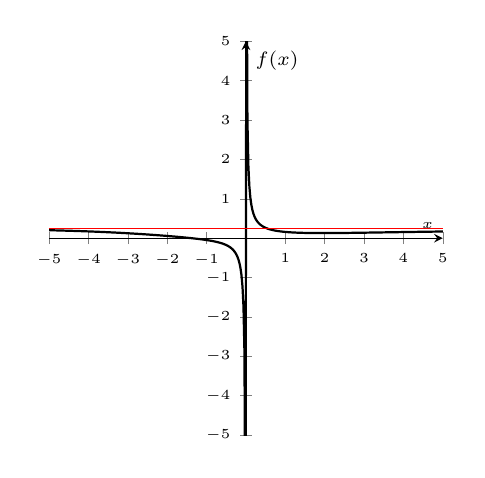
\begin{tikzpicture}
\begin{axis}[
]
\addplot[thick, samples=400] (x,{(3*x^3+x^2+8*x+17)/(12*x^3+17*(x^2+9*x))});
\addplot[samples=400,red] (x,3/12);
\end{axis}
\end{tikzpicture}
\subsubsection{پیوستگی}
پیوستگی یک نقطه در تابع، به معنی پیوسته بودن و قطع نشدن تابع در آن نقطه است. سه شرط زیر به ترتیب باید رعایت شوند تا بگوییم تابع در نقطه ی $a$ پیوسته است:
\begin{latin}
\begin{enumerate}
    \item $f(a) = L$
    \item $\lxa f(x) = L'$
    \item $L = L'$
\end{enumerate}
\end{latin}

\section{درس های جدید}
\subsection{اعداد مختلط}
عدد مختلط، ترکیبی از یک عدد موهومی \footnote{عدد موهومی(imaginary): $i=\sqrt[]{-1}$} و یک عدد طبیعی است.
که به $a$ مولفه حقیقی و به $b$ مولفه موهومی گفته میشود.
یک عدد مختلط معمولا به صورت زیر تعریف میشود: 
\[z = a + bi\]
\subsubsection{فرم قطبی}
یک عدد مختلط را میتواند به صورت قطبی هم نوشت. دستگاه زیر را در نظر بگیرید. $r$ فاصله نقطه از مبدا و $\theta$ زاویه نسبت به محور مثبت $x$ بر حسب رادیان است.

\begin{tikzpicture}[
     z={(0cm,0cm)},x={(0.5cm,0cm)},y={(0cm,0.5cm)},        % cavalier axes 
%  x={(-0.86cm,-0.5cm)},y={(0.86cm,-0.5cm)},z={(0cm,1cm)}  % isometric axes
  ]
  % x,y,z
  \def\ha{10}  % A height
  \coordinate (O) at (0,0,0);
  \def\a{5}
  \def\b{4}
  \draw[-latex] (O) -- (\ha,0,0) node [right]  {$x$};
  \draw[-latex] (O) -- (0,\ha,0) node [right] {$y$};
  \draw[->] (O) -- node [below] {$r$} (\a,\b,0) node [right] {$z=x+yi$};
  \draw[->] (1,0) to[out=0,in=-20] node [right] {$\theta$} (\a/5,\b/5);
\end{tikzpicture}

هنگام کار با اعداد مختلط فرض میکنیم $r$ مثبت است و $\theta$ می تواند هر زاویه ممکنی (مثبت و منفی) باشد. این بدین معنی است که بینهایت انتخاب برای تعیین $\theta$ وجود دارد. البته $z = 0$ از این قاعده مستثنی است. زیرا $\theta$ در مبدا تعریف نشده است. بنابراین، فرم قطبی را برای اعداد مختلط غیر صفر در نظر میگیریم.
فرمول تبدیل زیر را می توان برای تبدیل نقطه ای با مختصات قطبی $(r,\theta)$ به متخصات کارتزین $(x,y)$ به کار برد:
\[a=r\cos\theta\;\;\;\;\;\;\;\;\;\;\;\;\;b=r\sin\theta\]
اگر عدد مختلط را $z=a+bi$ تعریف کنیم، شکل قطبی آن به صورت زیر خواهد بود:
\[z=r(\cos\theta + i\sin\theta)\]
فرمول های زیر را میتوان برای تبدیل مختصات کارتزین به قطبی و نمایی استفاده کرد:
\[r=\sqrt{x^2+y^2}\]
مقدار $r$ در حقیقت همان اندازه $z$ است و می توان عدد مختلط را به صورت زیر هم نوشت:
\[z=|z|(\cos\theta+i\sin\theta)\]
زاویه $\theta$، آرگومان $z$ نام دارد و به صورت زیر نوشته میشود:
\[\theta=\arg z\]
آرگومان $z$ میتواند یکی از بی نهایت مقدار $\theta$ باشد که از حل رابطه زیر به دست می آید:
\[\tan\theta=\frac{y}{x}\]
که در نتیجه:
\[\theta=\tan^{-1}\frac{y}{x}\]

این تعداد آرگومان بی نهایت، به اندازه ضریب صحیحی از $2\pi$ با هم تفاوت دارند.

گفتیم برای انتخاب آرگومان یک عدد مختلط، بی نهایت انتخاب وجود دارد و همه این انتخاب ها به اندازه $2\pi$ نسبت به هم اختلاف دارند.
به عبارت دیگر، اگر $\theta$ پاسخ برای آرگومان عدد مختلط باشد، مقدار $\theta+2\pi$ نیز یک پاسخ است، زیرا به اندازه یک دور کامل در خلاف جهت عقربه های ساعت حرکت کرده و به همان نقطه $\theta$ رسیده است.
\subsubsection{فرم نمایی}
از فرمول اویلر استفاده میکنیم:
\[e^{i\theta} =\cos{\theta}+i\sin{\theta}\]
بعد با استفاده از فرمول اویلر میتوانیم فرم قطبی یک عدد مختلط را به فرم نمایی زیر بنویسیم:
\[z=re^{i\theta}\]
که در آن، $\theta=\arg{z}$ است و مشابه فرم قطبی، بی نهایت فرم نمایی برای یک عدد مختلط وجود دارد.
\subsection{عدد نپر (اویلر)}
عدد نپر به صورت زیر تعریف میشود:
\[e=\sum_{n=0}^{\infty} \frac{1}{n!}\]
لگاریتمی
{$\overset{\ref{subsec:log}}{}$}
 که مبنای آن عدد نپر باشد را به صورت زیر تعریف میکنیم: 
\[\log_e (x) = \ln (x)\]
\subsection{توابع هایپربولیک}
توابع هایپربولیک توابعی هستند که بجای دایره ی مثلثاتی به نسبت دو هذلولی افقی واحد متانسب میشوند.
 
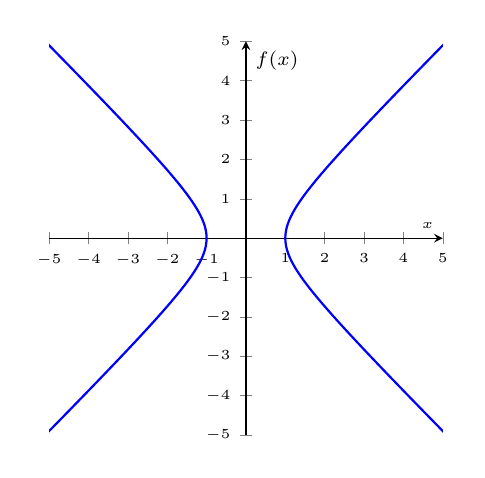
\begin{tikzpicture}
    \begin{axis}[]
        \addplot [blue,thick,samples=200] ({cosh(x)}, {sinh(x)});
        \addplot [blue,thick,samples=200] ({-cosh(x)}, {sinh(x)});
    \end{axis}
\end{tikzpicture}

نسبت های مثلثاتی هایپربولیک مثل نسبت های مثلثاتی معمولی تعریف و نوشته میشوند، ولی جلوی آنها حرف h برای هایپربولیک بودن می آید.

در توابع هذلولی افقی داریم $x^2 - y^2 = 1$ و میدانیم کسینوس هایپربولیک با ایکس و سینوس هایپربولیک با ایگرگ در رابطه ای که گفته شد متناسب است.
پس اتحاد مثلثاتی اول را در توابع هایپربولیک به صورت زیر مینویسیم: 
\[\cosh^2 x - \sinh^2 x = 1\]
\subsubsection{اتحاد های مثلثاتی هایپربولیک}
\begin{latin}
\begin{itemize}
    \item $\cosh^2 x - \sinh^2 x = 1$
    \item $\tanh x = \frac{\sinh x}{\cosh x}$
    \item $\coth x = \frac{\cosh x}{\sinh x}$
    \item $\sinh x = \frac{e^x - e^{-x}}{2}$
    \item $\cosh x = \frac{e^x + e^{-x}}{2}$
    \item $\tanh x = \frac{e^x - e^{-x}}{e^x + e^{-x}}$
    \item $\coth x = \frac{e^x + e^{-x}}{e^x - e^{-x}}$
    \item $\csch x = \frac{ 2 }{ e^x - e^{ -x } }$
    \item $\sech x = \frac{ 2 }{ e^x + e^{ -x } }$
    \item $\sinh(x \pm y) = \sinh x\cos y \pm \cosh x\sinh y$
    \item $\cosh(x \pm y) = \cosh x\cosh y \pm \sinh x\sinh y$
    \item $\tanh(u \pm v) = \frac{ \tanh u \pm \tanh u }{ 1 \pm \tanh u\tanh v }$
    \item $\tanh u * \coth u = 1$
    \item $\sech u = \frac{1}{ \cosh u }$
    \item $\csch u = \frac{1}{\sinh u }$
    \item $1-\tanh^2x = \sech^2x$
    \item $1-\coth^2x = -\csch^2x$
\end{itemize}
\end{latin}
\end{document}